\documentclass[border=8pt]{standalone}
\usepackage{amsmath,amssymb}
\usepackage{tikz}
\usetikzlibrary{arrows.meta,calc,decorations.pathreplacing,patterns,shapes.geometric,positioning,shadings,decorations.pathmorphing}

\begin{document}
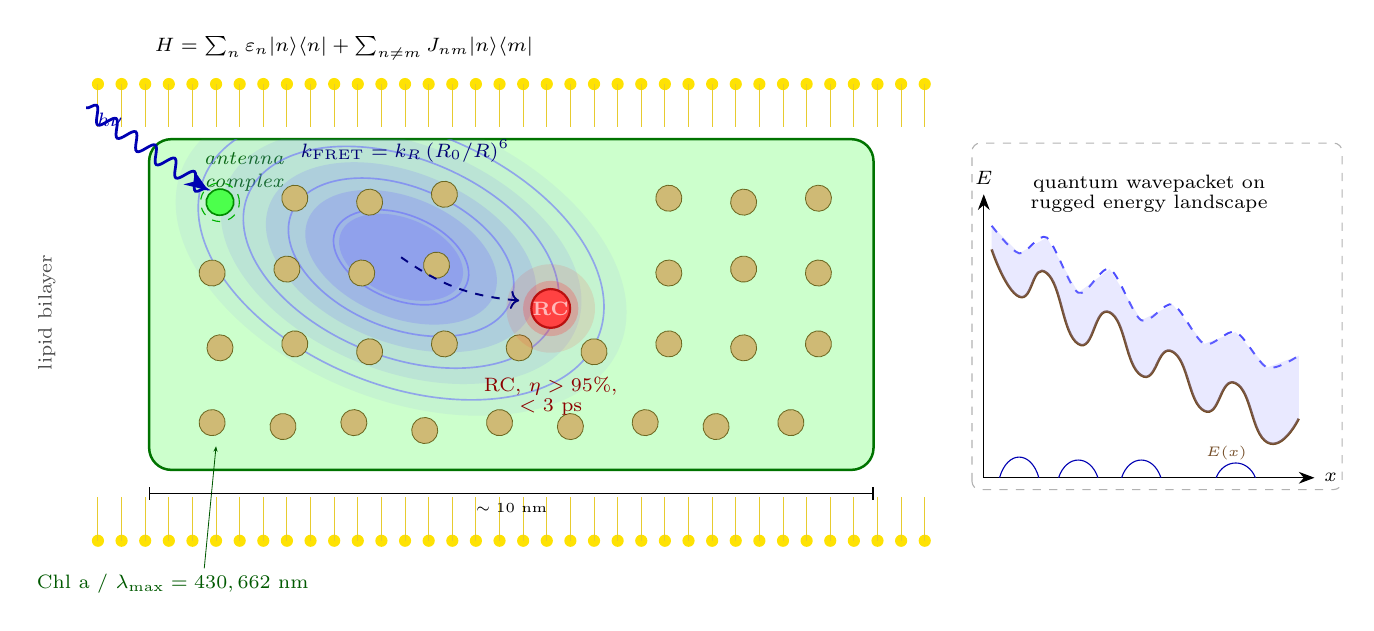
\begin{tikzpicture}[
    font=\small,
    pigment/.style={ellipse, minimum width=7pt, minimum height=4pt, draw=olive!70!black, fill=olive!40!brown!60, line width=0.3pt},
    photon/.style={blue!70!black, line width=1pt, decorate, decoration={snake, amplitude=1mm, segment length=3mm}},
    wave/.style={blue!60, line width=0.6pt, opacity=0.55},
    rc/.style={circle, minimum size=14pt, draw=red!60!black, fill=red!70, line width=0.8pt},
]

% ==== Lipid bilayer (top and bottom) ====
\foreach \x in {-0.25,0.05,...,10.3}{
    \fill[yellow!85!orange] (\x,5.6) circle (2.2pt);
    \draw[yellow!60!brown, line width=0.35pt] (\x,5.6) -- (\x,5.05);
    \fill[yellow!85!orange] (\x,-0.2) circle (2.2pt);
    \draw[yellow!60!brown, line width=0.35pt] (\x,-0.2) -- (\x,0.35);
}
\node[blue!40!black, font=\scriptsize] at (10.75,5.6) {};
\node[font=\scriptsize, gray!60!black, rotate=90] at (-0.9,2.7) {lipid bilayer};

% ==== Protein scaffold (antenna complex) ====
\draw[rounded corners=8pt, fill=green!20!white, draw=green!45!black, line width=0.9pt]
    (0.4,0.7) rectangle (9.6,4.9);
\node[font=\scriptsize\itshape, green!40!black] at (1.6,4.65) {antenna};
\node[font=\scriptsize\itshape, green!40!black] at (1.6,4.35) {complex};

% ==== Exciton wavepacket (blue wavy envelope going from upper-left toward center) ====
% Gaussian-like envelope drawn as concentric elongated ellipses
\begin{scope}
    \clip[rounded corners=8pt] (0.4,0.7) rectangle (9.6,4.9);
    \foreach \r/\op in {2.0/0.08, 1.6/0.12, 1.2/0.18, 0.85/0.25, 0.55/0.32}{
        \fill[blue!55, opacity=\op, rotate around={-22:(3.6,3.4)}]
            (3.6,3.4) ellipse (\r*1.5 and \r*0.9);
    }
    % wavefront ripples
    \foreach \rr in {0.6,1.0,1.4,1.8}{
        \draw[wave, rotate around={-22:(3.6,3.4)}] (3.6,3.4) ellipse (\rr*1.5 and \rr*0.9);
    }
\end{scope}

% ==== Pigment array (Chl molecules) ~ 24 ellipses in a lattice-ish arrangement ====
\foreach \x/\y/\r in {
    1.2/1.3/15, 2.1/1.25/-10, 3.0/1.3/20, 3.9/1.2/-5, 4.85/1.3/10, 5.75/1.25/-20, 6.7/1.3/5, 7.6/1.25/15, 8.55/1.3/-10,
    1.3/2.25/-20, 2.25/2.3/10, 3.2/2.2/-15, 4.15/2.3/5, 5.1/2.25/20, 6.05/2.2/-10, 7.0/2.3/15, 7.95/2.25/-5, 8.9/2.3/10,
    1.2/3.2/10, 2.15/3.25/-15, 3.1/3.2/5, 4.05/3.3/-10, 7.0/3.2/20, 7.95/3.25/-10, 8.9/3.2/5,
    1.3/4.1/-15, 2.25/4.15/10, 3.2/4.1/-5, 4.15/4.2/15, 7.0/4.15/-15, 7.95/4.1/5, 8.9/4.15/-20
} {
    \node[pigment, rotate=\r] at (\x,\y) {};
}

% Highlighted (excited) outer pigment
\node[ellipse, minimum width=10pt, minimum height=6pt, draw=green!55!black, fill=green!70, line width=0.6pt, rotate=10] (excited) at (1.3,4.1) {};
\draw[green!70!black, dashed, line width=0.4pt] (excited) circle (7pt);

% ==== Incoming photon (blue snake) ====
\draw[photon, -{Stealth[length=3mm]}] (-0.4,5.3) -- (1.15,4.25);
\node[blue!70!black, font=\scriptsize] at (-0.1,5.15) {$h\nu$};

% ==== Reaction center ====
\node[rc] (RC) at (5.5,2.75) {};
\node[font=\scriptsize\bfseries, white] at (RC) {RC};
\fill[red!80, opacity=0.25] (5.5,2.75) circle (10pt);
\fill[red!80, opacity=0.12] (5.5,2.75) circle (16pt);

% Arrow indicating focusing to RC
\draw[->, blue!50!black, line width=0.7pt, dashed] (3.6,3.4) to[bend right=15] (5.1,2.85);

% ==== Labels / formulas ====
\node[green!35!black, font=\scriptsize, align=left] at (0.7,-0.75)
    {Chl a / $\lambda_{\max}=430,662$ nm};
\draw[green!35!black, -{Stealth[length=2pt]}, line width=0.3pt] (1.1,-0.55) -- (1.25,1.0);

% Hamiltonian near scaffold
\node[anchor=west, font=\scriptsize] at (0.35,6.05)
    {$H=\sum_{n}\varepsilon_n|n\rangle\langle n|+\sum_{n\neq m} J_{nm}|n\rangle\langle m|$};

% FRET rate above wavepacket
\node[anchor=west, font=\scriptsize, blue!45!black] at (2.2,4.75)
    {$k_{\text{FRET}}=k_R\,(R_0/R)^6$};

% RC annotation
\node[anchor=north, font=\scriptsize, red!55!black, align=center] at (5.5,2.0)
    {RC, $\eta>95\%$,\\[-1pt] $<3$ ps};

% Scale bar (~10 nm)
\draw[|-|, line width=0.4pt] (0.4,0.4) -- (9.6,0.4);
\node[font=\tiny] at (5.0,0.22) {$\sim 10$ nm};

% ==== Inset: Energy landscape E(x) ====
\begin{scope}[shift={(11.0,0.6)}, scale=1.0]
    \draw[-{Stealth[length=2mm]}] (0,0) -- (4.2,0) node[right, font=\scriptsize] {$x$};
    \draw[-{Stealth[length=2mm]}] (0,0) -- (0,3.6) node[above, font=\scriptsize] {$E$};

    % Rugged energy landscape (smooth bumpy curve)
    \draw[brown!60!black, line width=0.9pt, smooth, tension=0.9]
        plot coordinates {
            (0.1,2.9) (0.45,2.3) (0.8,2.6) (1.2,1.7)
            (1.6,2.1) (2.0,1.3) (2.4,1.6) (2.8,0.85)
            (3.2,1.2) (3.6,0.45) (4.0,0.75)
        };

    % Wavepacket dashed envelope above the landscape (exploring many minima)
    \draw[blue!70, dashed, line width=0.7pt, smooth]
        plot coordinates {
            (0.1,3.2) (0.45,2.85) (0.8,3.05) (1.2,2.35)
            (1.6,2.65) (2.0,2.0) (2.4,2.2) (2.8,1.7)
            (3.2,1.85) (3.6,1.4) (4.0,1.55)
        };
    % Fill between: soft wavepacket band
    \fill[blue!40, opacity=0.22]
        plot coordinates {
            (0.1,3.2) (0.45,2.85) (0.8,3.05) (1.2,2.35)
            (1.6,2.65) (2.0,2.0) (2.4,2.2) (2.8,1.7)
            (3.2,1.85) (3.6,1.4) (4.0,1.55)
        } --
        plot[smooth, tension=0.9] coordinates {
            (4.0,0.75) (3.6,0.45) (3.2,1.2) (2.8,0.85)
            (2.4,1.6) (2.0,1.3) (1.6,2.1) (1.2,1.7)
            (0.8,2.6) (0.45,2.3) (0.1,2.9)
        } -- cycle;

    % Small wavepacket bumps indicating probability density
    \foreach \xc/\h in {0.45/0.35, 1.2/0.3, 2.0/0.3, 3.2/0.25}{
        \draw[blue!70!black, line width=0.4pt]
            (\xc-0.25,0) .. controls (\xc-0.15,\h) and (\xc+0.15,\h) .. (\xc+0.25,0);
    }

    \node[font=\scriptsize, anchor=south] at (2.1,3.5) {quantum wavepacket on};
    \node[font=\scriptsize, anchor=south] at (2.1,3.25) {rugged energy landscape};
    \node[font=\tiny, brown!60!black, anchor=south west] at (2.7,0.1) {$E(x)$};
\end{scope}

% Inset frame
\draw[rounded corners=3pt, dashed, gray!60] (10.85,0.45) rectangle (15.55,4.85);

\end{tikzpicture}
\end{document}
